\clearpage
\section{Flujo del sistema}
En esta sección vamos a describir de forma general el flujo que se debe seguir cualquier usuario cuando interactué con el sistema y que se puede ver en la figura .
\begin{figure}[H]
    \begin{center}
        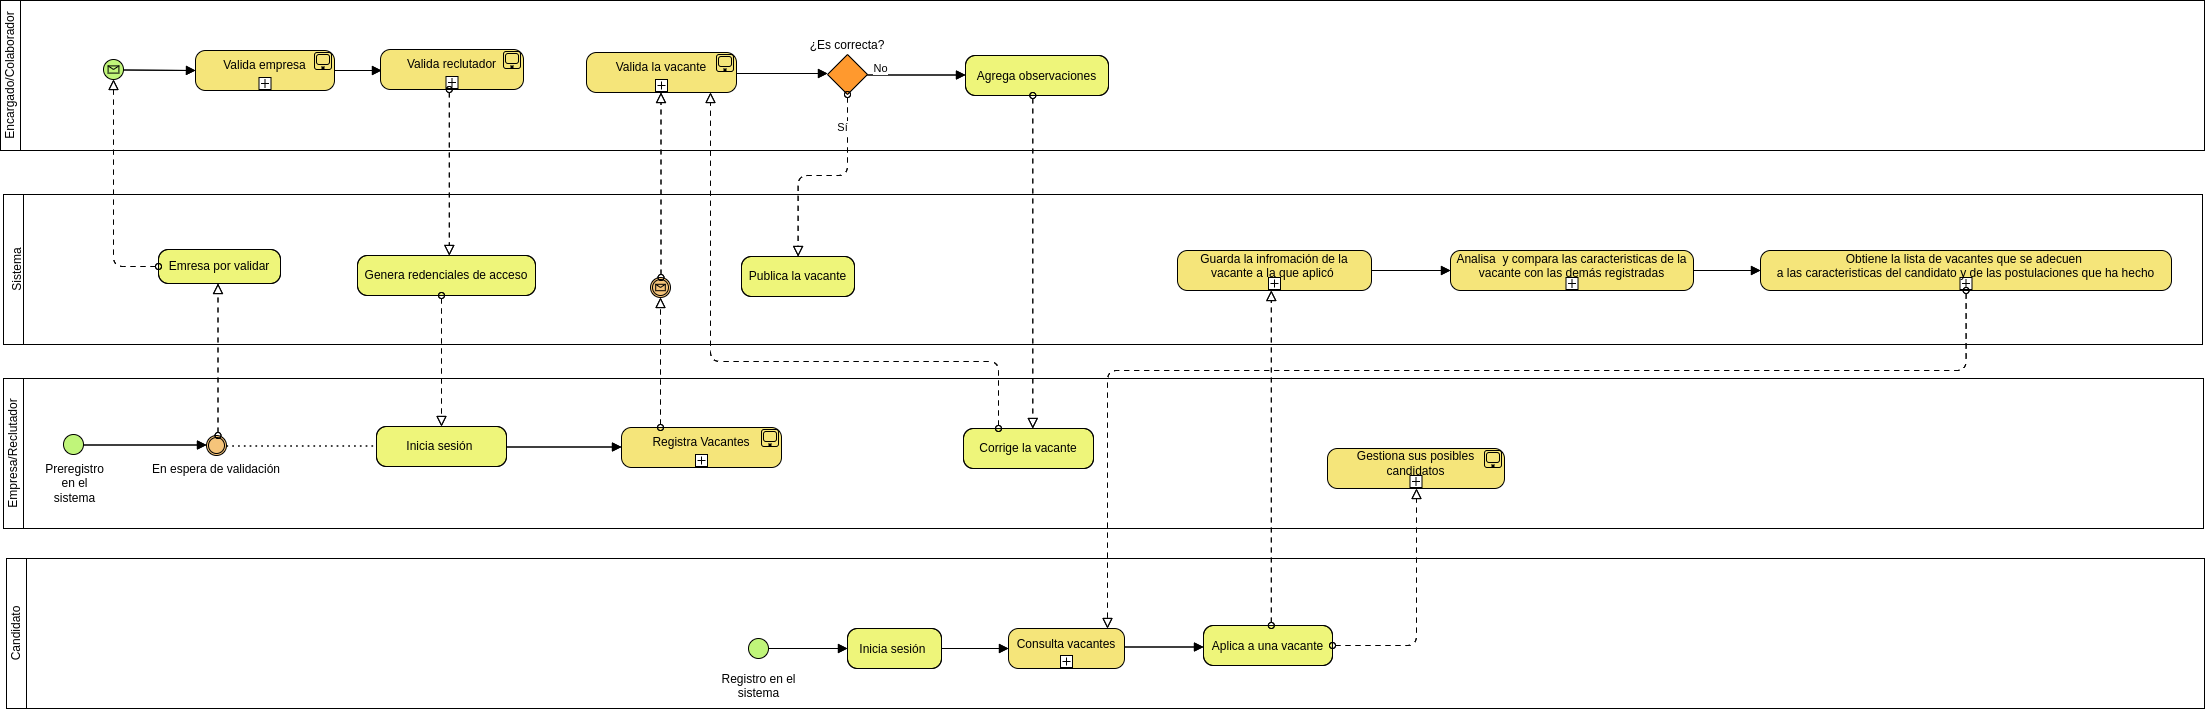
\includegraphics[height=0.27\textheight,angle=90]{propuesta/imagenes/Flujo.png}
    \end{center}
    \caption{Flujo del sistema.}
    \label{mark:top}
\end{figure}


Por negocio se identificaron 4 usuarios que pueden interactuar con el sistema:
\begin{itemize}
    \item \refElem{aCandidato}
    \item \refElem{aReclutador}
    \item \refElem{aColaborador}
    \item \refElem{aEncargado}
\end{itemize} 

DIchos actores estarán participando en 4 procesos importantes del sistema, a continuación se describen de manera breve dichos procesos:
\begin{itemize}
    \item Gestión de usuarios: en esta etapa se registran y validan reclutadores y empresas y si es necesario el encargado del sistema puede registrar más colaboradores dentro del sistema.\\Se puede tener más de un reclutador por empresa siempre y cuando sea validado por en encargado o colaborador del sistema.\\Solo existe un encargado en el sistema y solo el podrá registrar más colaboradores.
    \item Gestión de vacantes: en este proceso los reclutadores que hayan sido validados por el encargado y/o el mismo encargado del sistema podrán registrar vacantes. Sí el reclutador registra una vacante, esta tiene que ser validada por el encargado o colaborador del sistema, en dado caso que el colaborador encuentre detalles en la vacante podrá enviar observaciones al reclutador que haya creado la vacante y en consecuencia el reclutador la podrá corregir las veces que sean necesarias hasta que el encargado/colaborador le de visto bueno. Una vacante aprobada por el encargado/colaborador será publicada inmediatamente en el sistema. 
    \item Gestión de postulaciones: en este proceso los reclutadores podrán consultar loas perfiles de los candidatos que se hayan postulado a sus vacantes publicadas, asi como los candidatos recomendados para decidir quien continua con el proceso de postulación para la oferta o quien es descartado del proceso.% cabe recalcar que por cuestiones de privacidad y de negocio el reclutador solo podrá consultar los perfiles de l
    \item Recomendación de vacantes/candidatos: esta etapa es interna del sistema, cada vez que un candidato se postula a una vacante el sistema guarda la información de dichas postulaciones que el candidato haya hecho. Dichos datos son almacenados y comparados para hacer el proceso de recomendación tomando en cuenta dos factores:
    \begin{itemize}
        \item Las características del candidato que tiene registradas en su perfil y las de las vacantes que hay en el sistema registradas.
        \item Las características de las vacantes que el candidato se haya postulado y las de las vacantes que hay en el sistema registradas.
    \end{itemize} 
\end{itemize} 